% !TEX root = dissertation_BB.tex
%% spellcheck-language en-US

%    #
%   #
%  #  #
%  #####
%     #

\chapter{Real-time, GPU accelerated image processing pipeline}

\graphicspath{{./figures/4_gpu/}}


\section{GPU architecture}

\section{Live fusion}
  \subsection{MuVi-SPIM}
  \subsection{Bead based registration}

\section{B³D image compression}
  \b3d image compression
  B³D image compression

  \subsection{Data sizes in microscopy}

    \begin{figure}[tpb]
      \centering
      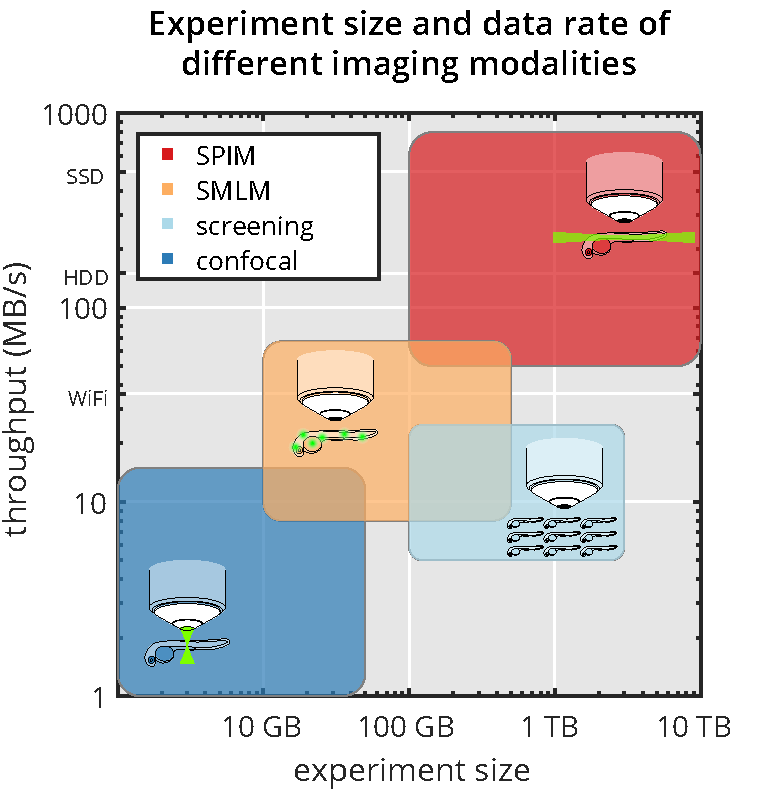
\includegraphics[page=1,width=0.6\textwidth]{comparison_with_pictograms}
      \bcaption[Experiment sizes and data rate of different imaging modalities.]{Comparison of single-plane illumination microscopy (SPIM, red rectangle), high-content screening (light blue), single molecule localization microscopy (SMLM, orange) and confocal microscopy (blue) by typical experiment size and data production rate (see also Table \ref{tab:sizes}).}
      \label{fig:sizes}
    \end{figure}


    \begin{table}[tbp]
      \begin{small}
        \renewcommand{\arraystretch}{2}
        \centering
        \begin{tabular}{rp{5cm}cccc}
            & \textbf{imaging device} & \textbf{image size} &  \parbox[c]{1.2cm}{\textbf{frame}\\ \textbf{rate}} & \textbf{data rate} & \parbox[c]{1.2cm}{\textbf{data\\ size}} \\
            \hline
            \hline
            \textbf{SPIM} & 2x sCMOS camera (e.g. Hamamatsu ORCA Flash4.0) & 2048x2048 & 50/s & 800 MB/s & 10 TB \\ \hline
            \textbf{SMLM} & 2x EMCCD camera (e.g. Andor iXon Ultra 897) & 512x512 & 56/s & 56 MB/s & 500 GB \\ \hline
            \textbf{screening} & CCD camera (e.g. Hamamatsu ORCA-R2) & 1344x1024 & 8.5s/ & 22 MB/s & 5 TB \\ \hline
            \textbf{confocal} & Zeiss LSM 880, 10 channels & 512x512 & 5/s & 12.5 MB/s & 50 GB \\ 
        \end{tabular}
        \bcaption[Data sizes in microscopy]{Typical devices used for confocal microscopy, high-content screening, single-molecule localization microscopy and light-sheet microscopy and their data production characteristics. Data visualized on Figure \ref{fig:sizes}}
        \label{tab:sizes}
      \end{small}
    \end{table}

  \subsection{Lossless compression performance}

    \begin{figure}[tpb]
      \centering
      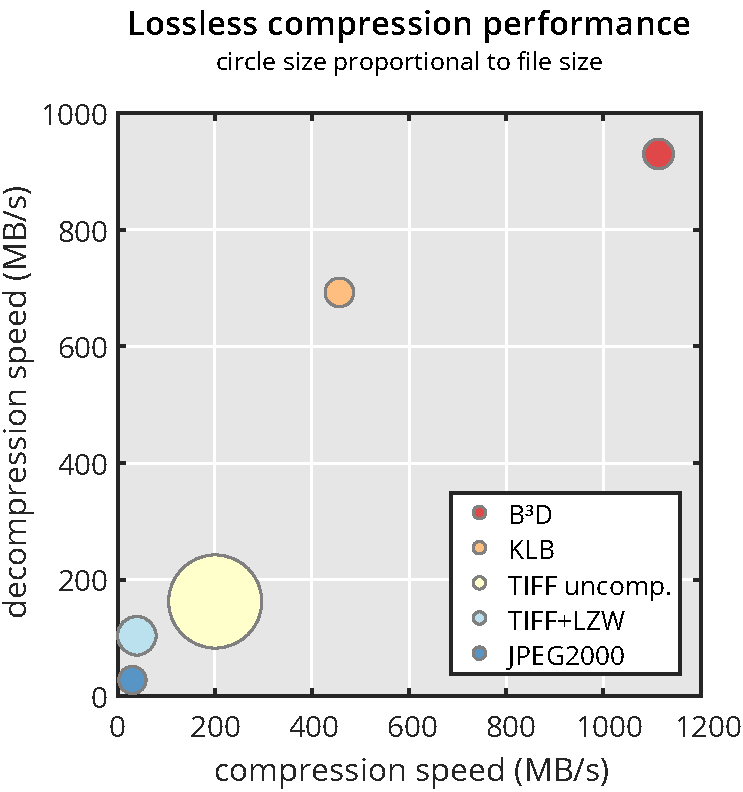
\includegraphics[page=1,width=0.6\textwidth]{bubbles}
      \bcaption[Lossless compression performance]{Performance comparison of our B³D \b3d compression algorithm (red circle) vs. KLB (orange), uncompressed TIFF (light yellow), LZW compressed TIFF (light blue) and JPEG2000 (blue) regarding write speed (horizontal axis), read speed (vertical axis) and file size (circle size). (see also Table \ref{tab:performance}).}
      \label{fig:performance}
    \end{figure}

    \begin{table}[tbp]
      \renewcommand{\arraystretch}{2}
      \setlength{\tabcolsep}{9pt}
      \centering
      \begin{tabular}{lrrrr}
          & \textbf{write speed} & \textbf{read speed} & \textbf{CR} & \textbf{file size} \\
          \hline
          \hline
          \textbf{\b3d} & 1,115.08 MB/s & 928.97 MB/s & 9.861 & 100\% \\ \hline
          \textbf{KLB} & 283.19 MB/s & 619.95 MB/s & 10.571 & 93.28\% \\ \hline
          \textbf{JPEG2000} & 31.94 MB/s & 26.38 MB/s & 11.782 & 83.69\% \\ \hline
          \textbf{JPEG2000} & 202.32 MB/s & 161.08 MB/s & 1.00 & 986.1\% \\ \hline
          \textbf{TIFF + LZW} & 40.85 MB/s & 102.37 MB/s & 5.822 & 169.37\%
      \end{tabular}
      \bcaption[Lossless compression performance]{\b3d is compared with various popular lossless image compression methods regarding write speed, read speed and compression ratio (original size / compressed size). Data visualized on Figure \ref{fig:performance}.}
      \label{tab:performance}
    \end{table}

  \subsection{Benchmarking}

    \begin{figure}[tpb]
      \centering
      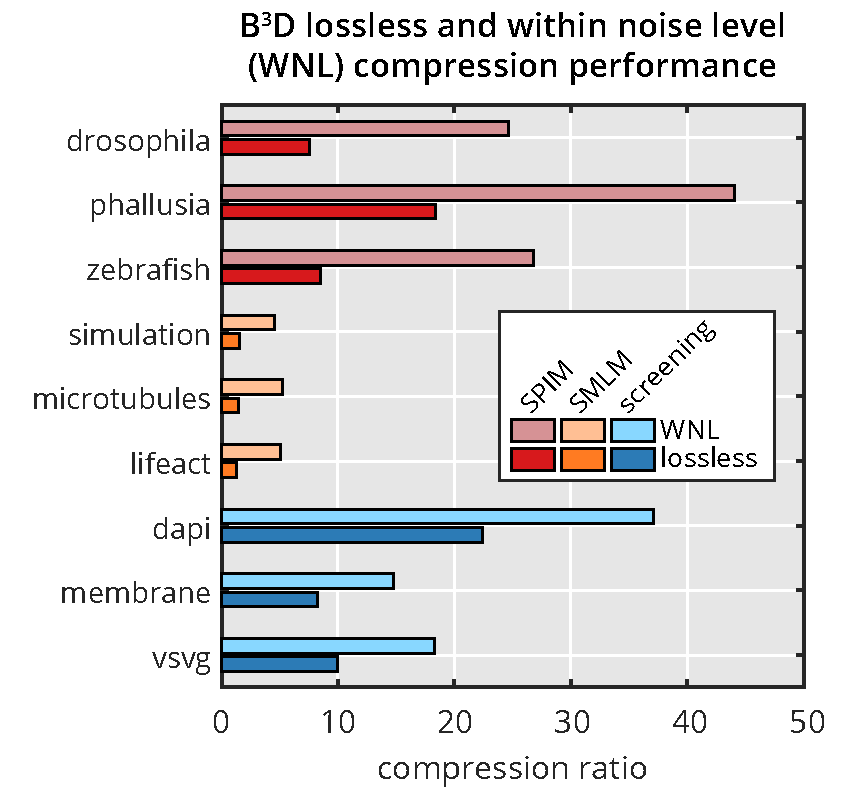
\includegraphics[page=1,width=0.6\textwidth]{Fig1c_compressionBars}
      \bcaption[Within noise level compression performance.]{For description of datasets see Table \ref{tab:datasets}.}
      \label{fig:benchmark}
    \end{figure}

    \begin{table}[tbp]
      \begin{small}
        \renewcommand{\arraystretch}{2}
        \centering
        \begin{tabular}{llp{7cm}r}
          \textbf{Dataset name} & \parbox[c]{2cm}{\textbf{Imaging\\modality}} & \textbf{Description} & \textbf{Size (MB)} \\
          \hline
          \hline
          \textbf{drosophila} & SPIM & dataset acquired in MuVi-SPIM of a Drosophila melanogaster embryo expressing H2Av-mCherry nuclear marker & 494.53 \\ \hline
          \textbf{zebrafish} & SPIM & dataset acquired in MuVi-SPIM of a zebrafish embryo expressing b-actin::GCaMP6f calcium sensor & 2,408.00 \\ \hline
          \textbf{phallusia} & SPIM & dataset acquired in MuVi-SPIM of a Phallusia mammillata embryo expressing PH-citrine membrane marker & 1,323.88  \\ \hline
          \textbf{simulation} & SMLM & MT0.N1.LD-2D simulated dataset of microtubules labeled with Alexa Fluor 647 from SMLMS 2016 challenge & 156.22 \\ \hline
          \textbf{microtubules} & SMLM & microtubules immuno-labeled with Alexa Fluor 674-bound antibodies in U2OS cells & 1,643.86  \\ \hline
          \textbf{lifeact} & SMLM & actin network labeled with LifeAct-tdEOS in U2OS cells & 3,316.15  \\ \hline
          \textbf{dapi} & screening & wide field fluorescence images of DAPI stained HeLa Kyoto cells \cite{simpson_genome-wide_2012} & 1,005.38 \\ \hline
          \textbf{vsvg} & screening & wide field fluorescence images of CFP-tsO45G proteins in HeLa Kyoto cells \cite{simpson_genome-wide_2012} & 1,005.38  \\ \hline
          \textbf{membrane} & screening & wide field fluorescence images of membrane localized CFP-tsO45G proteins labeled with AlexaFluor647 in HeLa Kyoto cells \cite{simpson_genome-wide_2012} & 1,005.38  \\ 
        \end{tabular}
        \bcaption[Datasets used for benchmarking compression performance]{}
        \label{tab:datasets}
      \end{small}
    \end{table}

\section{Noise dependent lossy compression}

\section{Methods}
